% Toda línea que comienza con un "%" es ignorada por LaTeX en la compilación. Esas líneas se llaman "comentarios".


%%%%%%%%%%%%% Definir la clase y los parámetros:
%Esto define la clase de documento que implica un cierto formato (tamaño de fuentes, tipo de numeración y títulos). Hay muchos formatos posibles. Cada revista científica tiene el suyo. Nosotros vamos a usar uno propio, cuyo archivo informeUNLP.cls fuente está subido al directorio de este 

% Elegir la codificación del textdocumento. Sin ese archivo, el documento no puede compilarse.

%%%% Si quieren el informe en una columna
%\documentclass[11pt,a4paper]{informeUNLP}

%%%% Si lo quieren en dos columnas
\documentclass[12pt,a4paper,twocolumn]{informeUNLP} %o según el SO: 
% Si usás Linux/FreeBSD (==MacOS)/Minix/Solaris 
\usepackage[utf8]{inputenc}
% Si usás Windows: 
%\usepackage[latin1]{inputenc}
\usepackage[spanish,es-tabla]{babel} %para que separe las palabras en español

%Más paquetes que hacen cosas, pueden googlear qué hace cada uno
\usepackage{multirow}
\usepackage{url} 
\usepackage{subfigure} 
\usepackage{xcolor}
\usepackage[centerlast,footnotesize]{caption} %cambia el tamaño de los captions
\usepackage{physics}
\usepackage{float}
\usepackage{amssymb}
\usepackage{amsmath}
\usepackage{inputenc}
\usepackage{enumitem}
\usepackage{hyperref}%Este paquete es muy importante porque convierte todas las referencias y citas en vínculos cliqueables.
\usepackage{booktabs}
\usepackage{tikz}
\usepackage[utf8]{inputenc}
  

\hypersetup{
    colorlinks=true,
    linkcolor=blue,
    filecolor=magenta,      
    urlcolor=black,
    citecolor=blue,
}%con este comando se puden elegir los colores de los vínculos que genera hyperref

%acá va el título y, si quieren, un subtítulo después de : 
\title{Confinamiento cuántico unidimensional: efecto de la longitud de conjugación en los niveles de energía de cianinas de las familias OXO y TIA.}

\author{Ignacio Montone, Braian Villalva, Damián  Mazzeo.\footnotemark[1]\\\textit{C\'atedra de Experimentos Cuánticos I,} \\\textit{Facultad de Ciencias Exactas, UNLP.}} %acá van les autores y las filiaciones

%\date{} %si queda vacío no podrá la fecha, se puede comentar esta línea y que ponga la última fecha de compilación o bien reemplazar con la fecha deseada

\begin{document}%el contenido del documento comienza acá
\twocolumn[
  \begin{@twocolumnfalse}
    \maketitle

    % el entorno "abstract" define la sección en la que se escribe el resumen del trabajo
  \begin{abstract}
Se estudió la dependencia de la longitud de onda de máxima absorción $\lambda_{\max}$, asociada a la transición electrónica HOMO $\rightarrow$ LUMO, con la longitud de la cadena conjugada $p$ en cianinas de las familias OXO (DOCI, DODCI, DOTCI) y TIA (DTCI, DTDCI, DTTCI). Se midieron los espectros de absorción UV-Vis de las OXO-cianinas en etanol y se emplearon los de las TIA-cianinas provistos por otro grupo; en todos los casos, $\lambda_{\max}$ se determinó ajustando una suma de dos gaussianas al pico principal de absorción. La relación entre $\lambda_{\max}$ y $p$ se ajustó con un modelo de pozo de potencial infinito y con uno de pozo finito, en el cual la altura de las paredes $V_0$ y la masa efectiva del electrón $m^*=\alpha m_e$ se dejaron como parámetros libres para cada familia. El ajuste con pozo finito arrojó $V_0 = 8,32(1)$ eV y $\alpha=0,81(1)$ para las OXO-cianinas, y $V_0=7,28(6)$ eV y $\alpha=0,86(2)$ para las TIA-cianinas, y describió los valores de $\lambda_{\max}$ de ambas familias con un acuerdo notablemente mejor que el pozo infinito.
\end{abstract}
\end{@twocolumnfalse}
]

%\footnotemark
%\footnotetext{nachomontone1@gmail.com, briantar437@gmail.com, mazzdami03@gmail.com}
%\begingroup
%\renewcommand{\thefootnote}{\fnsymbol{footnote}}
%\footnote{nachomontone1@gmail.com, briantar437@gmail.com, mazzdami03@gmail.com}
%\endgroup
% Solo el texto de la nota al pie, asociado al símbolo 1 (*)
{
  \renewcommand{\thefootnote}{\fnsymbol{footnote}}
  \footnotetext[1]{nachomontone1@gmail.com, briantar437@gmail.com, mazzdami03@gmail.com}
}
% Se puede habilitar la notación matemática escribiendo entre $$.
% El comando \section define una nueva sección en el artículo
\section{Introducción}

\subsection{Cianinas}
Los colorantes de polimetina (o metino) son moléculas cuyo cromóforo consiste en una cadena de dobles enlaces conjugados flanqueada por dos grupos terminales: un aceptor de electrones A y un donador de electrones D (Fig. \ref{fig:metino}) \cite{mishra2000}. Dentro de esta familia, las cianinas son las más difundidas. En ellas, ambos grupos terminales contienen un átomo de N, y el grupo amino o imino forma parte de un heterociclo; la carga positiva de la molécula se deslocaliza entre ambos N a lo largo de la cadena conjugada \cite{mishra2000,pronkin2015}.
\begin{figure}[H]
    \centering
    \includegraphics[width=1\linewidth]{figs/Methine_Dyes.jpg}
    \caption{Estructura de los colorantes de metino, con A aceptor y D donador.}
    \label{fig:metino}
\end{figure}

Según la naturaleza de los grupos terminales, las cianinas se clasifican en tres tipos (Fig. \ref{fig:cianina}) \cite{mishra2000}:
\begin{itemize}
    \item Streptocianinas o cianinas de cadena abierta (I), en las que ambos N son aminas sustituidas, no pertenecientes a un anillo:\\
    R$_2$N$^+$=CH[CH=CH]$_n$--NR$_2$.

    \item Hemicianinas (II), en las que uno de los N pertenece a un heterociclo y el otro es una amina abierta:\\
    Aryl=N$^+$=CH[CH=CH]$_n$--NR$_2$.

    \item Cianinas de cadena cerrada (III), en las que ambos N forman parte de anillos heterocíclicos:\\
    Aryl=N$^+$=CH[CH=CH]$_n$--N=Aryl.
\end{itemize}
\begin{figure}[H]
    \centering
    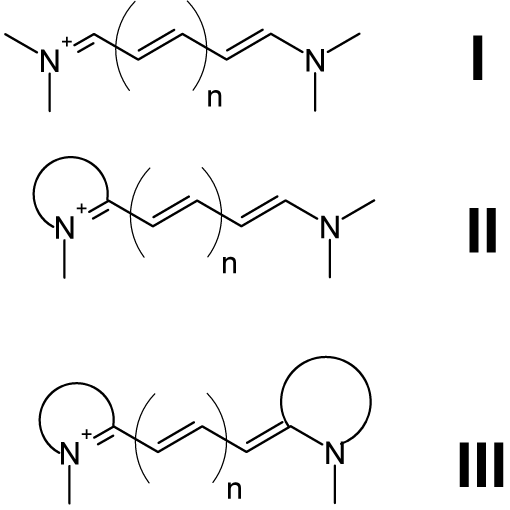
\includegraphics[width=0.7\linewidth]{Cyanine.png}
    \caption{Esquema estructural de los grupos de cianinas, con: I = Streptocianinas, II = Hemicianinas, III = Cianinas cerradas}
    \label{fig:cianina}
\end{figure}
De los tres tipos, el único relevante para este trabajo es el III, al cual pertenecen las oxo-cianinas y las tia-cianinas. Ambas familias comparten la misma estructura de dos heterociclos unidos por la cadena conjugada, y se diferencian únicamente por el heteroátomo presente en los anillos terminales: O (oxo) o S (tia) \cite{pronkin2015}.

\subsection{Estructura electrónica y transición HOMO$\rightarrow$LUMO}
\label{orbitas}
En la cadena conjugada, cada átomo aporta un orbital atómico $p$ perpendicular al plano de la molécula. El solapamiento lateral de estos orbitales genera orbitales moleculares $\pi$ deslocalizados a lo largo de toda la cadena (Fig. \ref{fig:orbitales}) \cite{medina2022}.

\begin{figure}[H]
    \centering
    \resizebox{\linewidth}{!}{%
    \begin{tikzpicture}
        % Esqueleto de la cadena: N - C - C - C - C - C - N
        \draw[thick] (0,0) -- (6,0);
        \foreach \x/\a in {0/N,1/C,2/C,3/C,4/C,5/C,6/N}{
            \fill[white] (\x,0) circle (0.2);
            \node at (\x,0) {\small \a};
            \fill[blue!40,opacity=0.7] (\x,0.65) ellipse (0.28 and 0.45);
            \fill[red!40,opacity=0.7] (\x,-0.65) ellipse (0.28 and 0.45);
            \draw (\x,0.65) ellipse (0.28 and 0.45);
            \draw (\x,-0.65) ellipse (0.28 and 0.45);
        }
        \node[anchor=east] at (-0.6,0.65) {\small (a)};
        % Orbital molecular pi deslocalizado
        \begin{scope}[yshift=-3cm]
            \draw[thick] (0,0) -- (6,0);
            \foreach \x/\a in {0/N,1/C,2/C,3/C,4/C,5/C,6/N}{
                \fill[white] (\x,0) circle (0.2);
                \node at (\x,0) {\small \a};
            }
            \fill[blue!40,opacity=0.7,rounded corners=10pt] (-0.35,0.2) rectangle (6.35,1.1);
            \fill[red!40,opacity=0.7,rounded corners=10pt] (-0.35,-0.2) rectangle (6.35,-1.1);
            \draw[rounded corners=10pt] (-0.35,0.2) rectangle (6.35,1.1);
            \draw[rounded corners=10pt] (-0.35,-0.2) rectangle (6.35,-1.1);
            \node[anchor=east] at (-0.6,0.65) {\small (b)};
        \end{scope}
    \end{tikzpicture}}
    \caption{Esquema de la formación de los orbitales $\pi$ en una cadena conjugada de $p=5$ átomos de C entre dos N. (a) Orbitales atómicos $p$ de cada átomo, perpendiculares al plano de la molécula; los colores indican el signo de la función de onda. (b) Al solaparse lateralmente, dan lugar a orbitales moleculares $\pi$ deslocalizados a lo largo de toda la cadena.}
    \label{fig:orbitales}
\end{figure}

Los electrones $\pi$ ocupan estos orbitales moleculares de menor a mayor energía. Se denomina HOMO (\textit{highest occupied molecular orbital}) al orbital de mayor energía que está ocupado, y LUMO (\textit{lowest unoccupied molecular orbital}) al de menor energía que está desocupado. Al absorber un fotón cuya energía coincide con la diferencia de energía $\Delta E_{H\rightarrow L}$ entre ambos orbitales, un electrón $\pi$ pasa del HOMO al LUMO. Esta es la transición electrónica fundamental ($\pi \rightarrow \pi^*$) \cite{pavia2014}, y en las cianinas corresponde a fotones del rango visible \cite{mishra2000}.

La energía $\Delta E_{H\rightarrow L}$ disminuye al aumentar la extensión de la conjugación, lo que produce un desplazamiento del máximo de absorción hacia longitudes de onda mayores \cite{pronkin2015}. Además, el átomo de S, al poseer una menor electronegatividad, mayor radio atómico y mayor polarizabilidad que el de O, favorece una mayor superposición con la cadena conjugada e incrementa la deslocalización de la densidad electrónica, lo que desplaza la absorción hacia energías menores en comparación con las oxo-cianinas análogas \cite{noukakis1995}.

Dado que el cromóforo absorbe luz visible y que los electrones $\pi$ están deslocalizados a lo largo de una cadena esencialmente unidimensional, la transición HOMO$\rightarrow$LUMO puede describirse con un modelo cuántico sencillo, en el que los electrones $\pi$ se tratan como partículas confinadas en un pozo de potencial unidimensional \cite{kuhn1949}.

\subsection{Espectroscopía UV-Vis}
La espectroscopía de absorción en la región ultravioleta-visible (UV-Vis) permite estudiar la estructura electrónica de una molécula a partir de la luz que esta absorbe \cite{skoog2017}. Un fotón es absorbido cuando su energía ($E = \frac{hc}{\lambda}$) coincide con la diferencia de energía entre dos estados de la molécula \cite{skoog2017}. El espectrofotómetro registra la absorbancia en función de la longitud de onda, y cada banda del espectro corresponde a una transición entre estados. En particular, la posición del máximo de la banda asociada a la transición HOMO$\rightarrow$LUMO, $\lambda_{\max}$, determina la diferencia de energía entre ambos orbitales, $\Delta E_{H\rightarrow L}=hc/\lambda_{\max}$. Esta es la magnitud que se compara con las predicciones de los modelos de confinamiento presentados a continuación.

\subsubsection{Ley de Beer-Lambert}
La determinación empírica de los espectros de absorción se fundamenta en la ley de Beer-Lambert, la cual establece una relación de proporcionalidad directa entre la atenuación luminosa y las propiedades macroscópicas del medio \cite{skoog2017}. La absorbancia espectral $A(\lambda)$ se define matemáticamente como:
$$A(\lambda) = \log_{10}\left(\frac{I_0}{I}\right) = \varepsilon(\lambda) l c$$
donde $I_0$ es la intensidad del haz incidente, $I$ es la intensidad de la radiación transmitida por la muestra, $\varepsilon(\lambda)$ es el coeficiente de absortividad molar característico de la especie química, $l$ es la longitud del paso óptico y $c$ es la concentración molar del analito \cite{skoog2017}.

Para que este modelo de proporcionalidad lineal sea válido, es un requisito fundamental operar en el régimen de disoluciones diluidas (típicamente inferiores a $0.01\text{ M}$) \cite{skoog2017}. A concentraciones elevadas, surgen dos tipos de desviaciones que invalidan la medición cuantitativa. Por un lado, las desviaciones por la menor distancia media entre las moléculas. Esta altera las interacciones electrostáticas y la distribución de carga de los analitos, modificando el valor intrínseco de su absortividad molar $\varepsilon(\lambda)$ \cite{skoog2017}. Por otro lado, las desviaciones instrumentales. Si la absorción es excesiva, la intensidad de radiación transmitida tiende al límite de detección del equipo ($I \to 0$), lo que produce una divergencia en el término logarítmico, satura el fotomultiplicador y rompe la linealidad de la respuesta.

\subsection{Pozo infinito}\label{intro:pozo_inf}
Por las particularidades mencionadas en la sección \ref{orbitas}, resulta adecuado modelar la diferencia de energía entre el HOMO y el LUMO considerando una partícula confinada en un pozo de potencial infinito. Entonces, tomando el potencial:
$$V(x) = \begin{cases}
0 & \text{si } -\frac{a}{2} \le x \le \frac{a}{2} \\[6pt]
\infty & \text{en otro caso}
\end{cases}$$
Y, la ecuación de Schrödinger \cite{griffiths2005}:
$$-\frac{\hbar^2}{2m} \frac{d^2 \psi(x)}{dx^2} + V(x)\psi(x) = E\psi(x)$$

Podemos encontrar una expresión para la energía discretizada $E_n$:
$$E_n=\frac{\hbar^2\pi^2}{2m_ea^2}n^2$$

Siendo $\hbar=\frac{h}{2\pi}$ con $h$ constante de Planck, $m_e$ masa del electrón, y $a$ el ancho del pozo (relacionado con el largo de la cadena de C).\\
Luego, notemos que cada átomo de C aporta un electrón $\pi$, y los dos N aportan tres en total, dando entonces $\pi_{tot}=N=p+3$ electrones $\pi$ presentes en la molécula, siendo $p$ el número de átomos de C de la cadena conjugada. Luego, por el principio de exclusión de Pauli, los orbitales ocupados son $n_{HOMO}=\frac{N}{2}=\frac{p+3}{2}$, por lo que, el primer orbital desocupado será $n_{LUMO}=\frac{N}{2}+1$. \\Por último, el ancho de la cadena $a$ se puede estimar conociendo la distancia interatómica de C conjugados $d=0,14$ nm \cite{roberts1977}, luego los C forman $p-1$ enlaces $\text{C}-\text{C}$ y los dos N juntos aportan el equivalente a $2 \times 1.5 = 3$ enlaces $\text{C}-\text{C}$. Quedando entonces $a=(p-1+3)d=(p+2)d$.\\
Ahora, con la expresión para $E_n$ y conociendo los valores de $n_{HOMO }$ y $n_{LUMO}$ podemos obtener:
$$\Delta E_{H\rightarrow L}=\frac{h^2}{8m_e((p+2)d)^2}(p+4)$$
Entonces, podemos obtener la longitud de onda $\lambda_{\max}$ asociada a esta diferencia de energía según la ecuación fundamental de la espectroscopía:
$$\Delta E=h\nu=\frac{hc}{\lambda}$$
dando entonces:
$$\lambda_{\max}=\frac{hc}{\Delta E_{H\rightarrow L}}=\frac{8m_ec((p+2)d)^2}{h(p+4)}$$
Observaciones: Este modelo predice un aumento lineal de la longitud de onda con el largo de la cadena. Sin embargo, no es posible diferenciar entre diferentes familias de cianinas. Esto último se toma como motivación para plantear un modelo que pueda describir la diferencia entre oxo-cianinas y tia-cianinas.

\subsection{Pozo finito} \label{intro:pozo_fin}
Consideremos nuevamente una partícula de masa $m$ confinada en la cadena, pero esta vez con paredes de altura finita $V_0$, asociada a los átomos extremos de la molécula. Esto permite que la función de onda penetre en las paredes y, como se verá, que el modelo distinga entre familias de cianinas. El potencial es
\[
V(x) =
\begin{cases}
V_0 & \text{si } x < -\frac{a}{2} \\
0   & \text{si } -\frac{a}{2} \le x \le \frac{a}{2} \\
V_0 & \text{si } x > \frac{a}{2}
\end{cases}
\]
y nos interesan los estados ligados, con $0<E<V_0$. La ecuación de Schrödinger independiente del tiempo \cite{griffiths2005} toma una forma distinta en cada región:
\begin{align}
\frac{d^2\psi}{dx^2} &= -k^2\psi \quad (|x|\le a/2), & k&=\frac{\sqrt{2mE}}{\hbar}, \\
\frac{d^2\psi}{dx^2} &= \kappa^2\psi \quad (|x|> a/2), & \kappa&=\frac{\sqrt{2m(V_0-E)}}{\hbar}.
\end{align}
Dentro del pozo las soluciones son oscilantes, mientras que fuera deben decaer exponencialmente para que $\psi$ sea normalizable, $\psi\propto e^{-\kappa|x|}$. Como $V(x)$ es simétrico respecto de $x=0$, las soluciones tienen paridad definida:
\begin{align*}
\text{pares:}\quad & \psi=A\cos(kx)\ \ (|x|\le a/2), & \psi&=Be^{-\kappa|x|}\ \ (|x|>a/2),\\
\text{impares:}\quad & \psi=A\sin(kx)\ \ (|x|\le a/2), & \psi&=\pm Be^{-\kappa|x|}\ \ (x\gtrless \pm a/2).
\end{align*}
Imponiendo que $\psi$ y $\psi'$ sean continuas en $x=a/2$ (la condición en $x=-a/2$ resulta equivalente por simetría) y dividiendo ambas condiciones entre sí, se obtiene
\begin{equation}
k\tan\!\left(\frac{ka}{2}\right)=\kappa \quad \text{(pares)},\qquad -k\cot\!\left(\frac{ka}{2}\right)=\kappa \quad \text{(impares)}.
\end{equation}
Introduciendo las variables adimensionales $v=ka/2$ y $u=\kappa a/2$, estas condiciones se escriben
\begin{equation}
u=v\tan v \quad \text{(pares)},\qquad u=-v\cot v \quad \text{(impares)},
\label{eq:empalme}
\end{equation}
mientras que, por las definiciones de $k$ y $\kappa$, ambas variables están vinculadas por
\begin{equation}
u^2+v^2=\frac{ma^2V_0}{2\hbar^2}\equiv z_0^2 \quad\Rightarrow\quad u=\sqrt{z_0^2-v^2}.
\label{eq:circ}
\end{equation}
La ecuación \eqref{eq:circ} depende solo de los parámetros del pozo ($m$, $a$, $V_0$), y la \eqref{eq:empalme} expresa el empalme de la función de onda con el exterior. Los niveles ligados son las intersecciones entre el arco de circunferencia \eqref{eq:circ} y las curvas \eqref{eq:empalme}; no admiten solución analítica, por lo que se calculan numéricamente. Hay un número finito de ellas, aproximadamente $2z_0/\pi$. Cada solución $v_n$ determina la energía del nivel
\begin{equation}
E_n=\frac{\hbar^2k^2}{2m}=\frac{2\hbar^2}{ma^2}\,v_n^2 .
\end{equation}
Ordenadas por energía creciente, las soluciones alternan entre pares e impares (el estado fundamental $n=1$ es par), con $v_n\in\left(\frac{(n-1)\pi}{2},\frac{n\pi}{2}\right)$. Para $V_0\to\infty$ resulta $v_n\to n\pi/2$, y se recupera la energía del pozo infinito.

Para obtener la energía de transición se usan los mismos niveles que en la sección \ref{intro:pozo_inf}, con $a=(p+2)d$: $n_{HOMO}=\frac{p+3}{2}$ y $n_{LUMO}=\frac{p+5}{2}$. Entonces
\[
\Delta E_{H\rightarrow L}=E_{n_{LUMO}}-E_{n_{HOMO}},\qquad \lambda_{\max}=\frac{hc}{\Delta E_{H\rightarrow L}},
\]
donde ambas energías se calculan para cada valor de $p$ resolviendo numéricamente \eqref{eq:empalme} y \eqref{eq:circ}. De esta manera, $\lambda_{\max}$ queda determinada por $V_0$ y por la masa $m$, que se tratan como parámetros a ajustar con los datos experimentales (sección \ref{sec:res_fin}).

\section{Materiales y métodos}

Se analizaron dos familias de colorantes: tia-cianinas (DTCI, DTDCI, DTTCI) y oxo-cianinas (DOCI, DODCI, DOTCI). Las mediciones experimentales de absorción óptica fueron realizadas por el grupo exclusivamente sobre las disoluciones de oxo-cianinas . Los espectros correspondientes a las  tia-cianinas fueron provistos por otro grupo de trabajo.

Las muestras se manipularon en disolución de etanol empleando cubetas de plástico y guantes de látex para evitar la contaminación. Las medidas se llevaron a cabo utilizando un espectrofotómetro UV/Vis de doble haz PerkinElmer Lambda 35, operando en la región de 200 nm a 900 nm, con un ancho de rendija de 1 nm, intervalos de medición de 1 nm y una velocidad de escaneo de 480 nm/min \cite{PerkinElmer}. El principio de funcionamiento óptico del equipo se detalla en la Figura \ref{fig:espectrofotometro}.

\begin{figure}[htbp] 
\centering
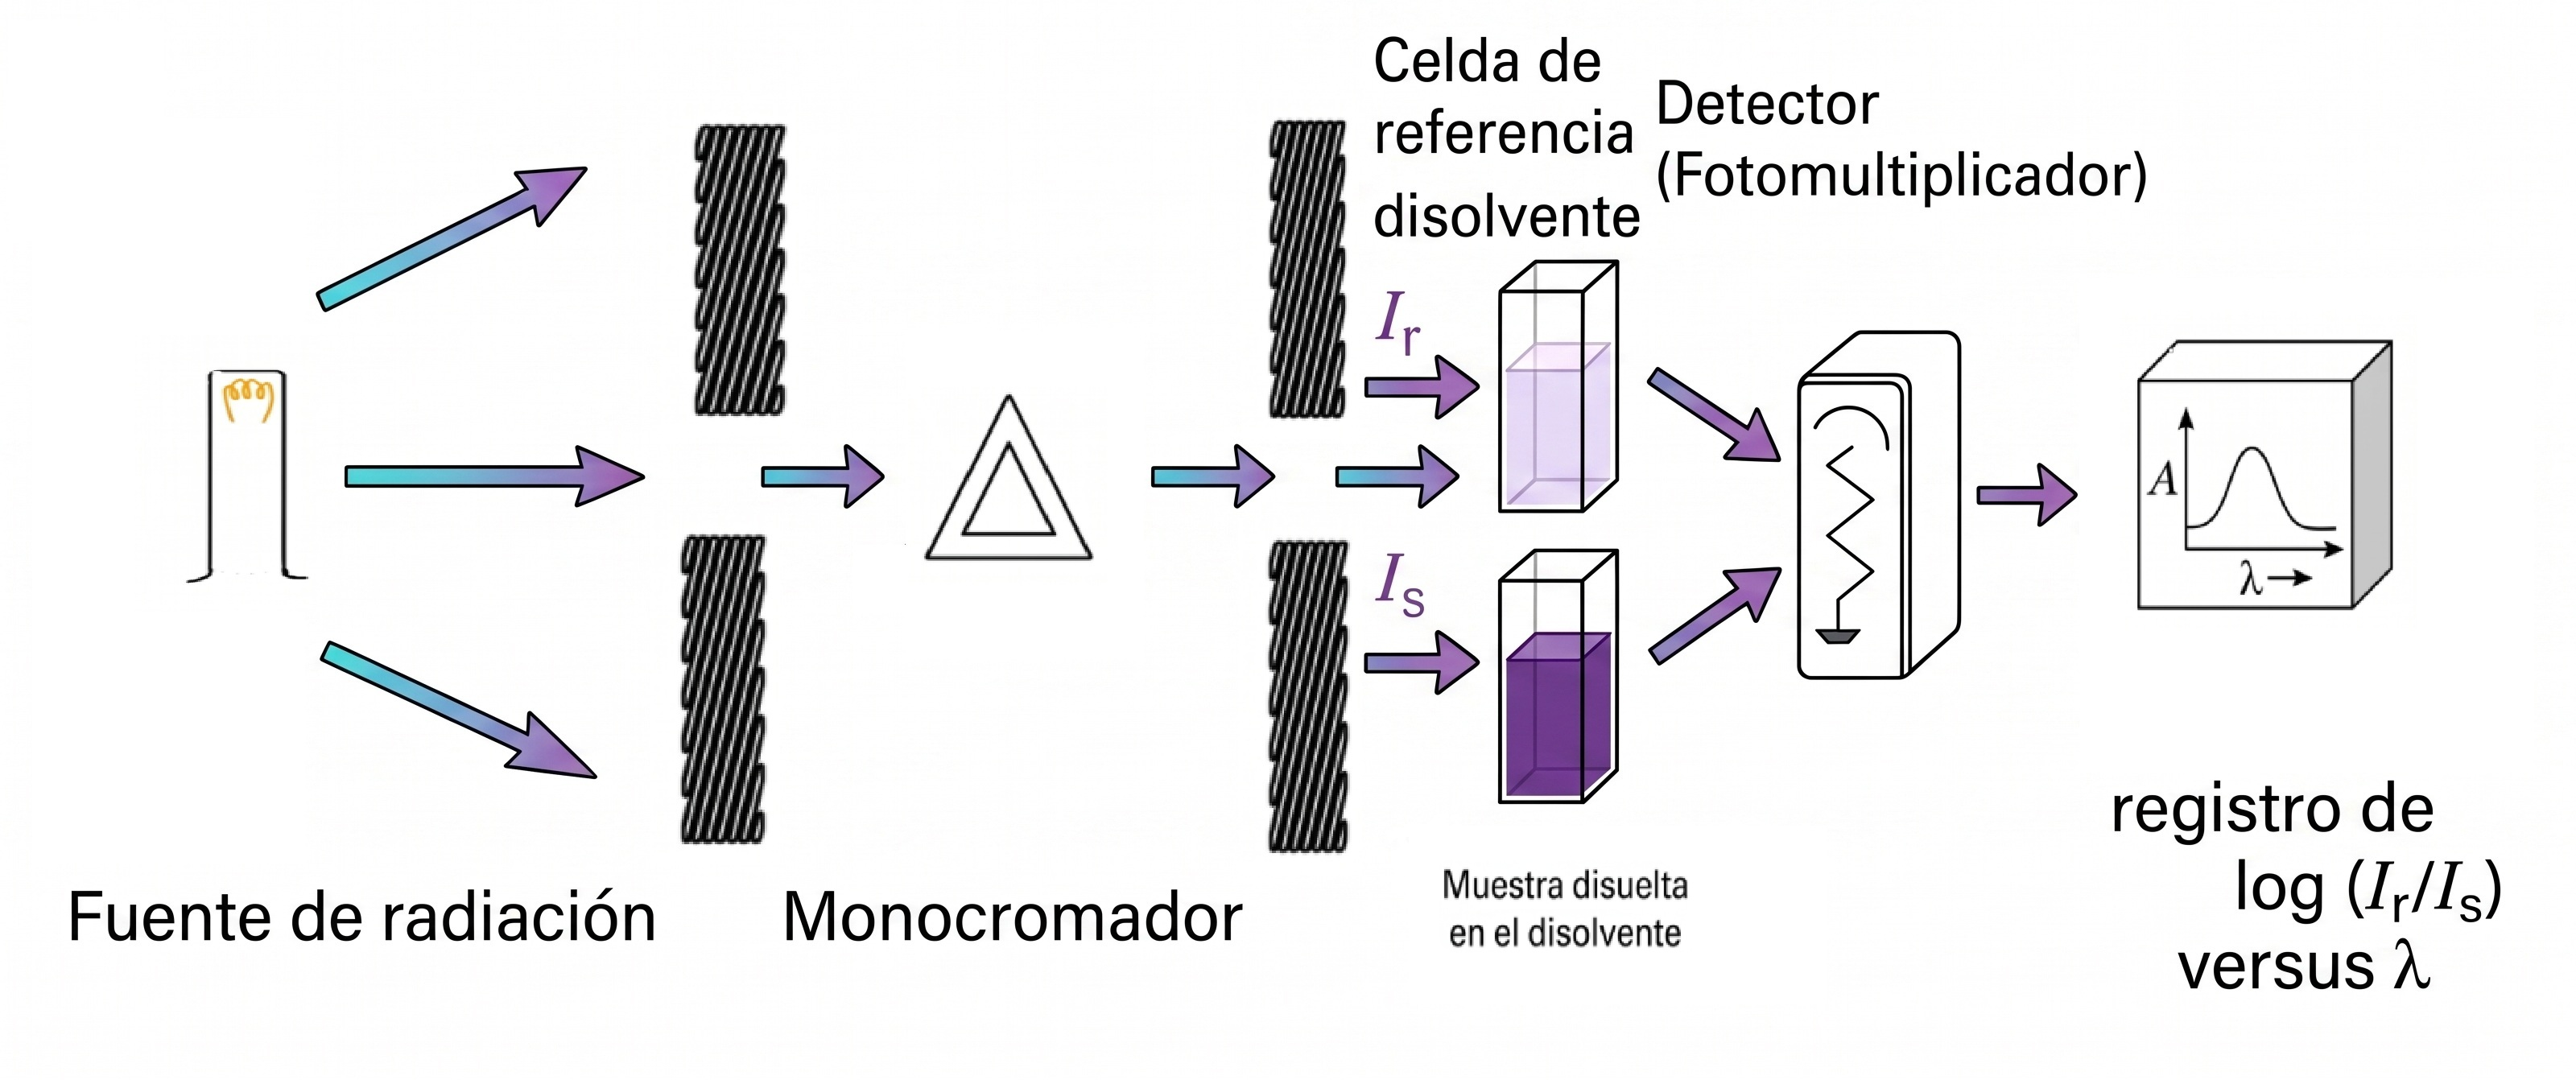
\includegraphics[width=\linewidth]{arreglo experimental.jpg}
\caption{Esquema de funcionamiento del espectrofotómetro UV-Vis de doble haz. El haz monocromático se divide para atravesar simultáneamente la celda de referencia (disolvente puro, $I_r$) y la celda con el analito ($I_s$). El sistema computa el espectro de absorbancia calculando la relación logarítmica de las intensidades transmitidas.}
\label{fig:espectrofotometro}
\end{figure}

El equipo fue operado mediante el software UV WinLab \cite{winlab}, el cual permitió la visualización en tiempo real de los espectros (absorbancia $A = \log(I_r/I_s)$ vs. $\lambda$) y la exportación de los datos. Inicialmente, se registró una línea base colocando cubetas con etanol puro en ambos haces del instrumento para corregir la absorción espectral del solvente y verificar la respuesta del detector. En esta instancia se detectó un funcionamiento irregular del instrumento (ruido excesivo) para $\lambda \lessapprox 280$ nm; sin embargo, al estar fuera de nuestra región espectral de interés, no afectó el análisis posterior.

Para la medición de las muestras, se colocó la disolución de cianina en la celda de medición manteniendo el etanol puro en la referencia. Se realizó un control de calidad espectral \textit{in situ}: si el espectro devuelto presentaba saturación del detector (picos aplanados) o valores de absorbancia muy superiores al rango lineal instrumental ($A \gg 1$), se procedia a diluir la muestra. Este procedimiento se repitió hasta obtener perfiles de absorción nítidos con máximos de absorbancia cercanos a $A = 1$, minimizando así el error relativo y garantizando la validez cuantitativa de la medición.

Finalmente, para los datos de absorbancia de ambas familias, se aisló la región correspondiente al pico principal de absorción y se realizó un ajuste empleando la suma de dos gaussianas. De este ajuste se extrajo el parámetro $\lambda_{\max}$, definido como la longitud de onda donde la absorción es máxima. %Estos valores fueron posteriormente se graficó $A$vs($p$) para su modelado cuántico.



%\section{Materiales y métodos}

%Contamos con 3 OXO-cianinas distintas, específicamente: DOCI (p=5), DODCI (p=7) y DOTCI (p=9), que se manipularon dentro de cubetas de vidrio con guantes de látex para evitar la contaminación.
%Se utilizó un espectrofotómetro PerkinElmer Lambda 35 UV/Vis en la región de 200 nm a 900 nm, de doble haz, con un ancho de rendija de 1 nm, saltos de 1 nm y una velocidad de escaneo de 480 nm/min \cite{PerkinElmer}. Conectado a una computadora con el software UV WinLab \cite{winlab} para la manipulación del mismo, visualización de gráficos ($\log\frac{I}{I_0}$ vs $\lambda$) y exportación de resultados.
% Habria que aclarar que tenia para poner 2 cubetas el equipo o se sobreentiende?

%Inicialmente, se midió con cubetas llenas de etanol para ambos haces, para obtener un gráfico base del instrumento y poder comprobar su correcto funcionamiento. 
%Luego se fue rellenando una cubeta con una cianina, mientras la otra se mantuvo con el etanol. Para este procedimiento, se rellenaba la cubeta con la cianina disuelta en una solución de alcohol, se medía y se revisaba el gráfico. Si el mismo devolvía picos cuadrados o valores mucho mayores a 1, se volvía a realizar la medición pero con las cianinas aún más disueltas en el alcohol, para evitar la saturación del instrumento y tener menor error relativo.

%Se midió con cada cianina hasta obtener picos suaves y con su máximo alrededor de 1.

%Una vez realizado el procedimiento para los 3 tipos de OXO-cianinas, se exportaron los datos y se procedió a manipularlos: en primera instancia se visualizó el gráfico base, donde se encontró un funcionamiento irregular del instrumento para $\lambda \lessapprox 280$ nm. Como nuestros picos de interés se encontraban fuera de esta zona, no se tuvo en cuenta y se prosiguió con el análisis normalmente. 


%Para los datos de cada cianina se recortó la zona de interés (pico de absorción), luego se realizó un ajuste de suma de 2 gaussianas y así se obtuvo el valor de $\lambda$ para el cual la absorción $A$ era máxima, que fue llamado $\lambda_{\max}$.
%Se realizó el mismo procedimiento con los datos de las TIA-cianinas compartidos.
%Por último se graficaron los datos de $\lambda_{\max}$ en función de $p$ con ambos grupos de cianinas. 



\section{Resultados}

\subsection{Análisis para el pozo infinito}
Una vez obtenidos los valores de $\lambda_{\max}$ para cada cianina (Tabla \ref{tab:infresult}), se realizó un gráfico $\lambda_{\max}$ vs $p$ con el objetivo de comparar ambas familias y hacer un ajuste con el modelo de pozo infinito (tratado en la sección \ref{intro:pozo_inf}). Se muestra en la Figura \ref{fig:pozo_inf}.
\begin{figure}[H]
    \centering
    \includegraphics[width=1\linewidth]{figs/pozo_inf.png}
    \caption{Gráfico de $\lambda_{\max}$ en función de $p$ para ambas familias de cianinas con el ajuste para el modelo de pozo infinito. Se observa una discrepancia entre el modelo y los datos, además de una diferencia entre ambas familias.}
    \label{fig:pozo_inf}
\end{figure}

Se observa que, para un $p$ dado, $\lambda_{\max}$ es menor para las oxo-cianinas. Por lo que en una cadena $\text{C}-\text{C}$ de igual longitud se espera un $\Delta E_{H\rightarrow L}$ mayor para las oxo-cianinas.



Luego, es notable que tal como se anticipó, el modelo no distingue entre tipos de familias y tampoco es coherente con los datos. Por estas razones se procedió a realizar un análisis similar para un modelo más adecuado.

\begin{table}[htbp]
    \centering
    \begin{tabular}{|p{1.5cm}|p{1.5cm}|p{1.5cm}|p{1.5cm}|}
        \hline
        % Encabezado / Fila 1
        Familia& Nombre & $\lambda_{\max}(nm)$  & $p$ \\ \hline
        
        % Grupo 1 (3 filas)
        \multirow{3}{*}{Oxo} & DOCI&485,1(1) &5 \\ \cline{2-4}
        & DODCI&582,56(3)&7 \\ \cline{2-4}
        & DOTCI& 686,98(3) &9 \\ \hline
        
        % Grupo 2 (3 filas, exactamente igual a Grupo 1)
        \multirow{3}{*}{Tia} & DTCI & 557,75(2) & 5 \\ \cline{2-4}
        & DTDCI& 642,72(2) & 7 \\ \cline{2-4}
        & DTTCI& 760,39(2) & 9\\ \hline
    \end{tabular}
    \caption{Valores de $\lambda_{\max}$ para cada cianina, con $p$ el número de enlaces conjugados en la cadena} 
    \label{tab:infresult}
\end{table}

\subsection{Análisis para el pozo finito}\label{sec:res_fin}
Para una mayor exactitud, se cambió a un modelo de \textbf{pozo finito} (sección \ref{intro:pozo_fin}). Dónde las paredes del pozo de potencial dejan de ser paredes impenetrables para el electrón, sino que este puede traspasarlas a un cierto potencial que llamamos $V_0$. También se añadió un factor de corrección a la masa del electrón, ya que el valor bibliográfico es el correspondiente a un electrón libre y en reposo; mientras que en la cianina se encuentran en estados ligados, por lo que su masa difiere. Se definió una masa efectiva $m^* = \alpha m_e$, con $V_0$ y $\alpha$ parámetros a ajustar. Los resultados obtenidos se encuentran en la figura \ref{fig:pozo_fin} y tabla \ref{tab:refini}.


\begin{figure}[h]
    \centering
    \includegraphics[width=1\linewidth]{figs/masa_eff.png}
    \caption{Gráfico de $\lambda_{\max}$ en función de $p$ para ambas familias de cianinas con el ajuste para el modelo de pozo finito. Se observa una mayor coherencia con los datos de ambas familias.}
    \label{fig:pozo_fin}
\end{figure}

\begin{table}[h!]
    \centering    
    \begin{tabular}{|p{2.5cm}|p{2.5cm}|p{2cm}|}
        \hline
        \textbf{Familia} & \textbf{\(V_0\) (eV)} & \textbf{\(\alpha\)} \\ \hline
        Oxo & 8,32(1) & 0,81(1) \\ \hline
        Tia & 7,28(6) & 0,86(2) \\ \hline
    \end{tabular}
    \caption{Valores de \(V_0\) y \(\alpha\) para cada familia mediante el ajuste de pozo finito y masa efectiva.}
    \label{tab:refini}
\end{table}


\section{Discusión y conclusiones}
Mediante la técnica de espectroscopia de UV-vis, se tomaron datos de A en función de $\lambda$ para oxo-cianinas(DOCI, DODCI, DOTCI) y tia-cianinas(DTCI, DTDCI, DTTCI). Luego se determinó el $\lambda_{\max}$ (tabla \ref{tab:infresult}) para cada una, asociado al diferencia de energía entre el HOMO y el LUMO. \\Con el objetivo de modelar esta transición elemental, se opto primeramente por un modelo cuántico sencillo: una partícula confinada en un pozo de potencial infinito. De este modo, se realizó un ajuste de los datos (figura \ref{fig:pozo_inf}) y se concluyó que no es coherente con los puntos experimentales. Sin embargo, si respeta la tendencia del corrimiento hacia el rojo. \\ 
%Luego, de una profunda depresión e insatisfacción por no poder representar la realidad de las cianinas mediante el modelo de pozo infinito, no quedó mas alternativa que considerar
Ante las discrepancias con los datos y la incapacidad del modelo de pozo infinito para diferenciar las familias de cianinas, se consideró
%se considero%
una partícula confinada en un pozo finito, con paredes de altura $V_0$ el cual fue un parámetro a determinar mediante un análisis numérico. A su vez, se introdujo un factor de corrección a la masa del electrón, se definió una masa efectiva $m^* = \alpha m_e$. Como se observa en la tabla \ref{tab:refini} este modelo distingue entre ambas familias y guarda una mejor correspondencia con los datos. Es notable que $V_{0}^{oxo}$ es mayor que $V_{0}^{tia}$, %debido a los efectos desarrollados en la sección \ref{orbitas}. \\
lo que evidencia que los electrones experimentan un mayor confinamiento en los extremos de la primera familia, que concuerda con la mayor electronegatividad y menor deslocalización del sistema $\pi$ del O respecto al S. \\
Para ambas familias se obtuvo $\alpha <1$ lo que evidencia que la interacción y solapamiento  entre orbitales adyacentes reduce la inercia de los electrones $\pi$ con respecto a los libres.\\
Como conclusión, podemos afirmar que el modelo de pozo finito es mas adecuado a la hora de describir las energías de transición de orbitales de los electrones de familias de cianinas, ya que los extremos de la molécula presentan un potencial finito que permiten la penetración de la función de onda de los electrones hacia los terminales. \\ Resultaría interesante extender el experimento a otras familias de cianinas cerradas, para observar si existe una tendencia monotónica del parámetro $\alpha$ con $V_0$.
%(DTCI, DTDCI, DTTCI) y oxo-cianinas (DOCI, DODCI, DOTCI)Se concluye que el modelo de pozo infinito no es suficiente para describir el salto orbital de los electrones en cianinas, y que contrario a lo que este modelo indica, si hay diferencias en las energías de salto entre ambas familias. Específicamente, este modelo arroja $\lambda_{\max}$ menores a los datos experimentales, lo que se traduce en una energía necesaria para el salto menor a la esperada por el modelo.

%Para el modelo de pozo finito se observa una correlación mucho más exacta a la de los datos experimentales, aunque este presenta un parámetro de ajuste $V_0$ que hace diferencia entre ambas familias. Para el caso de las OXO, se espera una pendiente mayor a la obtenida, mientras que en la familia TIA el modelo coincide con los datos.

%Como conclusión, podemos afirmar que el modelo de pozo finito es mucho más certero a la hora de describir las energías de transición de orbitales de los electrones de familias de cianinas, ya que los extremos de la molécula presentan un potencial finito que hacen que la probabilidad de que los electrones se encuentren allí sea no nula.


\bibliographystyle{unsrt}
\bibliography{LaBibliografia}{}  


\end{document}
